

\documentclass[a4paper, 12pt, oneside]{book}
\usepackage[left=2.5cm,right=2.5cm,top=2.5cm,bottom=2.5cm]{geometry}
\usepackage[spanish, es-noshorthands, activeacute]{babel} 
\usepackage[utf8]{inputenc}
\usepackage{graphicx}
\usepackage{subcaption} % para poner dos imágenes en una misma línea
\usepackage{amssymb}
\usepackage{amsthm}
\usepackage{amsmath}
\usepackage{makeidx}
\usepackage{color}
\usepackage{parskip}
\usepackage{multirow}
\usepackage{hyperref} % para poner hipervínculos en el PDF
%%%%%%%%%%%%%%%%%%%%%%%%%%%%%%%%%%%%%%%%%%%%%%%%%%%%%%%%%%%%%%%%%%%%
\newtheorem{definicion}{Definición}
\newtheorem{lema}{Lema}
\newtheorem{proposicion}{Proposición}
\newtheorem{teorema}{Teorema}
\newtheorem{corolario}{Corolario}
\newtheorem{observacion}{Observación}
\newtheorem{ejemplo}{Ejemplo}
\newtheorem{ejercicio}{Ejercicio}
%añadir [chapter] al final de cada comando si se desea que la numeración vaya acorde al capítulo

%%%%%%%%%%%%%%%%%%%%%%%%%%%%%%%%%%%%%%%%%%%%%%%%%%%%%%%%%%%%%%%%%%%%%
\renewcommand{\thesection}{\arabic{section}}
%%%%%%%%%%%%%%%%%%%%%%%%%%%%%%%%%%%%%%%%%%%%%%%%%%%%%%%%%%%%%%%%%%%%%




\begin{document}
\pagenumbering{roman}
%-------------------------------------------------------------------------Inicio P\'{a}gina del T\'{\i}tulo
\begin{titlepage}


\includegraphics[scale=0.18]{logo-facultad-ciencias-uma}

\vskip2truecm

\begin{center}

% Upper part of the page. The '~' is needed because \\
% only works if a paragraph has started.

%\includegraphics[width=0.35\textwidth]{\textbf{logo-facultad-ciencias-uma}}~\\[1cm]
 

%\textsc{\LARGE Universidad de M\'{a}laga}

%\textsc{Facultad de ciencias}\\ [1.5cm]

%\textsc{\Large Trabajo Fin de Grado}\\[0.5cm]

% Title
%\noindent\rule{\textwidth}{0.4mm}
{ \huge \bfseries T\'{\i}tulo del tfg en espa\~{n}ol  \\[0.4cm] }

%\noindent\rule{\textwidth}{0.4mm}
\vskip1truecm

{ \huge \bfseries T\'{\i}tulo del tfg en ingl\'es \\[0.4cm] }

%\noindent\rule{\textwidth}{0.4mm}


\vskip1truecm

{\Large Trabajo Fin de Grado en Matem\'aticas} \\

{\Large Universidad de M\'alaga} \\

%\vfill
\end{center}

\vskip2truecm

\noindent\rule{\textwidth}{0.4mm}

\vskip.2truecm


{\bf Autor:} {Guillermo Cascales Ñíguez}\\

{\bf \'{A}rea de conocimiento y/o departamento:} {Departamento de Análisis Matemático, Estadística e Investigación Operativa y Matemática Aplicada}  \\

{\bf Fecha de presentaci\'{o}n: (mes y a\~{n}o)}\\

{\bf Tema:}\\

{\bf Tipo:} {(trabajo de revisi\'on bibliogr\'afica, de iniciaci\'on a la investigaci\'on,...)}\\

{\bf Modalidad:} {(individual o grupal)}\\

{\bf N\'umero de p\'aginas (sin incluir introducci\'on, bibliograf\'{\i}a ni anexos):}\\




\end{titlepage}
%-------------------------------------------------------------------------Fin P\'{a}gina del T\'{\i}tulo
%----------------P\'agina en blanco--------------------------------------------------------------
\newpage
\mbox{}
\thispagestyle{empty}
%----------------Fin p\'agina en blanco---------------------------------------------------
\begin{titlepage}
\begin{center}



\textsc{\Large DECLARACI\'{O}N DE ORIGINALIDAD DEL TFG}\\[0.5cm]
\bigskip

%\noindent\rule{\textwidth}{0.4mm}
\vskip2truecm
% Author and tutor
%\begin{minipage}{0.4\textwidth}
%\begin{flushleft} \large
%\emph{Autor:}\\
%\textsc{Nombre y Apellidos del autor}
%\end{flushleft}
%\end{minipage}
\end{center}

D./D\~{n}a. \textit{(nombre del autor)}, con DNI (NIE o pasaporte) \textit{(DNI, NIE o pasaporte)}, estudiante del Grado en \textit{(titulaci\'{o}n)} de la Facultad de Ciencias de la Universidad de M\'{a}laga,\\
\textbf{DECLARO:}\\

Que he realizado el Trabajo Fin de Grado titulado ``\textit{(T\'{i}tulo)}'' y que lo presento para su evaluaci\'{o}n. Dicho trabajo es original y todas las fuentes bibliogr\'{a}ficas utilizadas para su realizaci\'{o}n han sido debidamente citadas en el mismo.\\
\medskip

De no cumplir con este compromiso, soy consciente de que, de acuerdo con la normativa reguladora de los procesos de evaluaci\'on de los aprendizajes del estudiantado de la Universidad de M\'alaga de 23 de julio de 2019, esto podr\'a conllevar la calificaci\'on de suspenso en la asignatura, sin perjuicio de las responsabilidades disciplinarias en las que pudiera incurrir en caso de plagio.
\bigskip


Para que as\'{i} conste, firmo la presente en M\'{a}laga, el \textit{(fecha)}\\



%\vfill

%\noindent\emph{Tutor y co-tutor (si lo hubiera):} \\
%{\bf Prof. Dr. Nombre y apellidos del tutor}
%\bigskip
%\bigskip
%\bigskip

%\noindent \emph{Palabras Clave:}\\
%\textsc{poner aqu\'{\i} las palabras clave.}

\vskip.3truecm
% Bottom of the page

\qquad\qquad\qquad {Fdo:..............................................................}

\end{titlepage}











\tableofcontents

\addcontentsline{toc}{chapter}{Resumen} 
\addcontentsline{toc}{chapter}{Abstract} 
\addcontentsline{toc}{chapter}{Introducci\'on}

\pagebreak

{\let\clearpage\relax

{\Large \textbf{El T\'{\i}tulo aqu\'{\i}}}\\

\chapter*{Resumen}
} 
Este Trabajo Fin de Grado se sitúa en el ámbito del aprendizaje automático
(Machine Learning). En particular, se analiza en profundidad la arquitectura de
las Redes Neuronales para luego ser aplicadas en el campo de la detección
de anomalías, encargado de encontrar patrones o eventos que se salgan de la
normalidad en un sistema.
En primer lugar, se analizan desde un enfoque teórico los elementos básicos
de la teoría del Machine Learning, como los de clasificador, función de pérdida,
error de entrenamiento y test, aprendizaje PAC, dimensión VC, red neuronal, función de activación o entrenamiento, de los que este trabajo se sirve para mostrar
los resultados y métodos centrales en este área como pueden ser el teorema
fundamental del aprendizaje PAC, el descenso de gradiente, la regularización o
los autoencodificadores.
Finalmente, el marco teórico desarrollado se ejemplifica experimentalmente
mediante una aplicación práctica sobre un dataset real de detección de fraude
en transacciones financieras con tarjetas de crédito.


\vfill

\textbf{Palabras clave:}\\

\textsc{Aprendizaje automático, Redes neuronales, Aprendizaje PAC,
Autoencodificadores, Detección de anomalías, Redes neuronales de replicación.
}

\pagebreak

{\let\clearpage\relax

{\Large \textbf{El T\'{\i}tulo (en ingl\'{e}s) aqu\'{\i}}}\\

\chapter*{Abstract}
}

Text. 

\vfill

\textbf{key words:}\\

\textsc{key words.}

\chapter*{Introducci\'on}
Desde tiempos inmemoriales, los humanos hemos soñado con crear una máquina
que fuese capaz de pensar. En cuanto aparecieron los primeros ordenadores, 
no tardamos mucho tiempo en imaginarnos un futuro con robots que tuvieran
capacidad de raciocinio, que pudiesen juzgar de la misma forma y facilidad
con la que una persona lo hace. 

En sus primeros días, la \textit{inteligencia artificial} (IA) resolvió 
rápidamente problemas intelectualmente complicados para los humanos. 
Por ejemplo, el ENIAC, uno de los primeros computadores de propósito general,
era capaz de calcular la potencia 660.000 de un número de 10 cifras en tan
sólo 1,5 segundos, y fue inicialmente diseñado para calcular tablas de tiro de
artillería destinadas al Laboratorio de Investigación Balística del Ejército de los Estados Unidos. 

Pero el verdadero reto no era resolver problemas que pudieran ser descritos 
mediante una lista de reglas matemáticas y formales, sino aquellas tareas 
que son sencillas y automáticas para las personas, como reconocer una cara 
o el lenguaje hablado, pero al mismo tiempo muy difíciles de describir formalmente.
Los primeros intentos de atacar a este problema se basaban principalmente en una serie de reglas.
En el caso de identificar lenguaje hablado, el algoritmo busca si la persona está
diciendo una letra en particular. Pero cada persona tiene un tono distinto, 
por lo que un conjunto
de reglas que buscase cada letra y se tuviese que 
adaptar al tono y acento del usuario, además de poco efectivo sería muy tedioso de elaborar.

En su lugar, podemos elaborar un algoritmo que no resolverá directamente la tarea, sino que 
usará datos extraídos previamente (en el ejemplo del reconocimiento de voz, serían numerosas grabaciones transcritas)
para así intentar \textit{aprender} el verdadero algoritmo, que se el que luego hará la
tarea de \textit{predicción}. En definitiva, tenemos dos fases: una primera \textit{fase de entrenamiento}
donde se aprende el algoritmo, y una segunda \textit{fase de predicción} en la que se use 
el algoritmo para resolver la tarea. Esta última fase de predicción suele ser más barata
computacionalmente a diferencia que la fase de entrenamiento, la cual es más lenta y necesita
de hardware de mayor potencia y coste.


De este modo, este trabajo se centra en la resolución de los problemas intuitivos, 
evitando que un operador humano se encargue de traducir a la máquina formalmente 
el conocimiento que necesita. En su lugar, centraremos los esfuerzos en hacer que 
el computador capture el conocimiento extrayendo patrones de datos en crudo, lo 
que se conoce como \textit{aprendizaje automático} (\textit{machine learning}).

El rendimiento de estos algoritmos de aprendizaje automático dependen enormemente 
de la \textit{representación} de los datos. Por ejemplo, si entrenamos un clasificador
que estime la probabilidad de que un paciente tenga cáncer de pulmón, el algoritmo no
examinará al paciente directamente. 
En cambio, el doctor extraerá una serie de \textit{características} del paciente, 
como su edad, si fuma o no, la densidad de los tejidos, la forma de los órganos,
etc., y el algoritmo será capaz de aprender patrones útiles para predecir
la probabilidad de que el paciente tenga cáncer de pulmón. 

Ahora bien, saber qué características en concreto extraer es una tarea complicada. Si 
queremos, por ejemplo, desarrollar un programa que detecte cápsulas de medicamentos defectuosas
en base a imágenes de estas, quizás podríamos buscar si tienen un agujero o si están chafadas. 
Sin embargo, describir cómo se ve un agujero o cuál es la forma de la cápsula en términos de valores de 
píxeles en una imagen es muy difícil, pues esta última se podría ver alterada por un texto
impreso en la pastilla, como ocurre en la \autoref{fig:capsules}.

\begin{figure}[htbp]
    \centering 
    
    \begin{subfigure}[b]{0.48\textwidth}
        \centering
        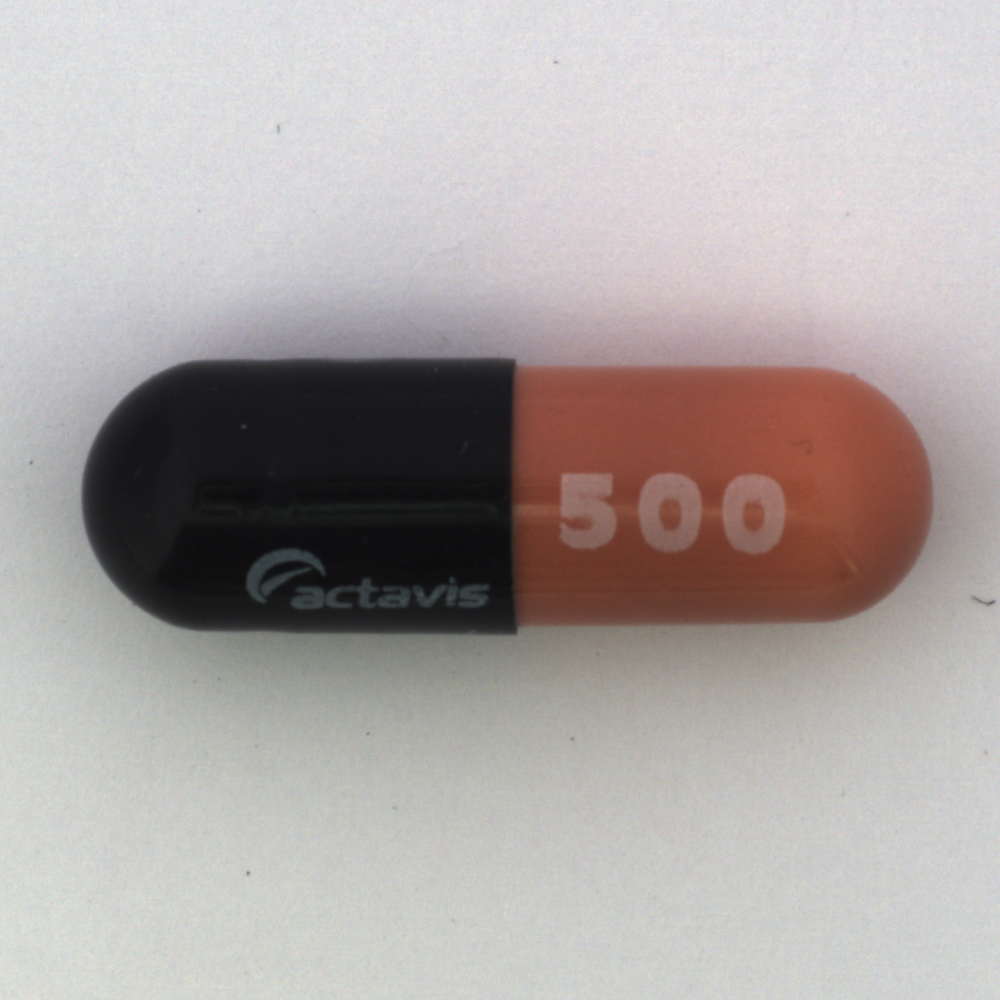
\includegraphics[width=0.6\linewidth]{images/capsule_good} 
        \caption{Cápsula en buen estado}
        \label{fig:capsule_good}
    \end{subfigure}
    \hfill 
    \begin{subfigure}[b]{0.48\textwidth}
        \centering
        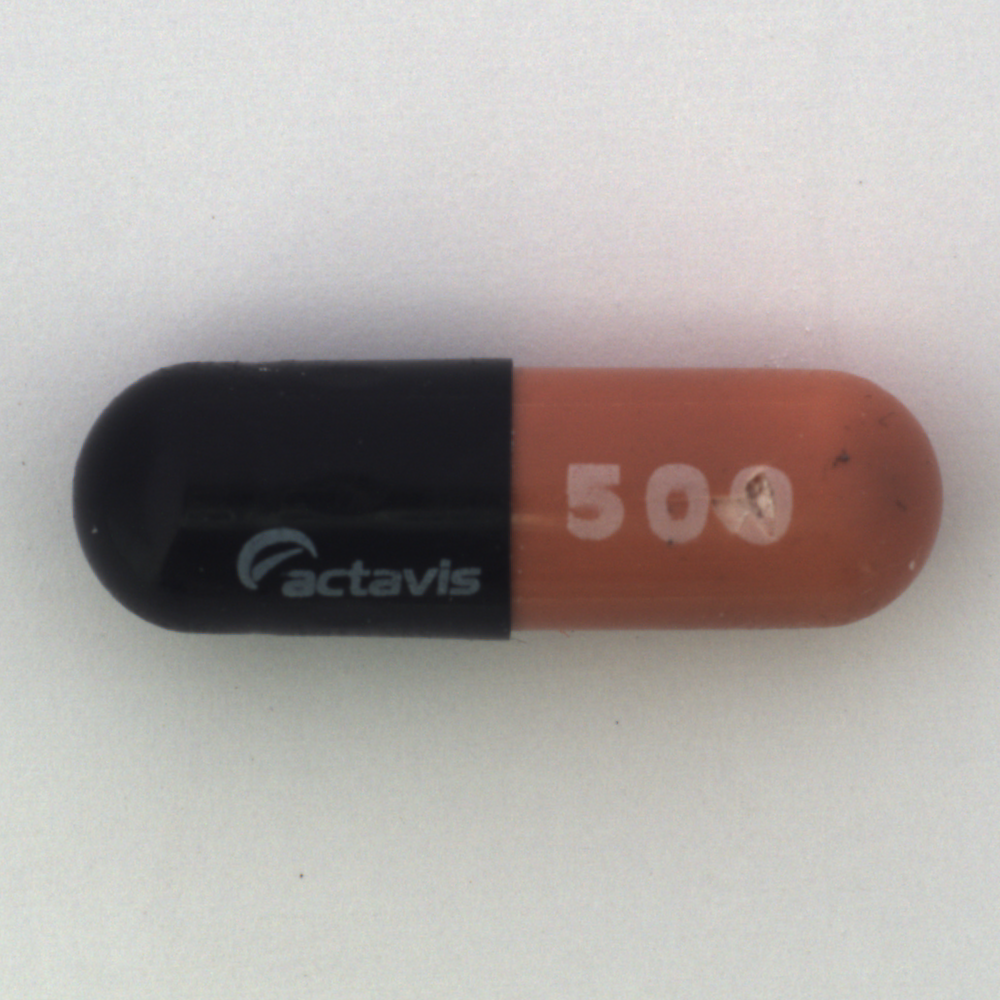
\includegraphics[width=0.6\linewidth]{images/capsule_bad.png} 
        \caption{Cápsula con una perforación}
        \label{fig:capsule_bad}
    \end{subfigure}

\caption{La detección del agujero en la cápsula se ve dificultada por la presencia de un texto
que tiene el mismo color.}
\label{fig:capsules}
\end{figure}

Una solución a este problema es usar el aprendizaje automático no sólo para devolver una 
clasificación en base a una representación, sino además para devolver dicha representación 
como tal. Esto se conoce como \textit{aprendizaje de características} (\textit{representation learning}).
Los \textit{autoencodificadores} (\textit{autoencoders}) son un ejemplo de representation learning.
Estos combinan un \textit{encodificador}, que transforma los datos de entrada en otra representación, para
luego usar un \textit{decodificador} que convierte esta nueva representación de vuelta en el formato
original. La idea es entrenar el autoencoder para que preserve la mayor cantidad de información
posible cuando reciba un input. El output también guarda ciertas propiedades, aunque de eso, y 
de los diferentes tipos de autoencoder se hablará más tarde.



\chapter{Introducción al aprendizaje automático}
\pagenumbering{arabic}
\setcounter{page}{1} 

Algunas de las tareas típicas que se trabajan en el machine learning son:

\begin{itemize}
    \item \textit{Clasificación estadística/Clasificación}: clasificar un \textit{input} en un número finito de \textit{clases}.
    Un ejemplo es el reconocimiento de voz, donde el input es el audio y las clases son las letras
    del abecedario (o las palabras del diccionario).
    \item \textit{Regresión}: se predice un valor numérico dada una entrada. Podría ser 
    el interés de un préstamo dadas las características del prestatario, o los costes 
    médicos anuales esperados que una aseguradora tiene que asumir.
    \item \textit{Detección de anomalías}: se detectan entradas fuera de la norma, como pueden ser,
    a modo de ejemplo, la detección de cápsulas defectuosas, errores en la pintura de un coche o 
    transacciones fraudulentas de tarjetas de crédito.
    \item \textit{Aprendizaje reforzado}: se entrena un agente para tomar la decisión correcta
    en cada momento según la situación, como hacen los robots de ajedrez o los coches autónomos
\end{itemize}

Entre muchas otras.

\section{Conceptos básicos}
En primer lugar, nos centraremos en la \textbf{clasificación estadística}. Nuestro objetivo es 
entrenar un clasificador que, dado un \textbf{input}, nos devuelva una \textbf{etiqueta} o 
\textbf{clase}. El ejemplo de clasificador por antonomasia es el \textit{OCR} (\textit{Optical Character Recognition}),
y, más concretamente, el reconocimiento de números escaneados. El \textbf{dataset} más
conocido es el  MNIST\footnote{NIST viene de National Institute of Standards and Technology, la agencia que recopiló estos datos. The M viene de "Modified", 
pues los datos fueron preprocesados para facilitar su uso en el machine learning.}, 
el ``Hello world''\footnote{O como Geoffrey Hinton, padrino de la IA diría, la \textit{drosophila}, en referencia a la mosca de la fruta que estudian los biólogos.} 
del aprendizaje automático, que contiene 70000 imágenes de números escritos a mano en formato 28x28 píxeles, i.e. tenemos un conjunto \(\mathcal{X} = \{0, 1, \dots , 255\}^{28
\times28}\subseteq   \mathbb{R}^{28\times28}  \)
que se conoce como \textbf{dominio}, en el cual viven nuestros datos, y queremos etiquetar correctamente, es decir, encontrar una función \(h\colon \mathcal{X} \to \mathcal{Y} \) llamada clasificador, 
con \(\mathcal{Y} \) el conjunto de etiquetas posibles (para el MNIST, \(\mathcal{Y} = \{1, 2, \dots , 9\}\) ). 
Se dice que estos datos (imágenes, en este caso) están \textbf{etiquetados}, pues la imagen por sí sola no le bastaría al algoritmo para aprender qué número es cual. 
Es lo que se conoce como \textit{aprendizaje supervisado} (\textit{supervised learning}). En contraposición, existen los algoritmos de \textit{aprendizaje no supervisado} 
(\textit{unsupervised learning}), los cuales se centran en aprender la distribución de los datos para así descubrir propiedades interesantes en la estructura de estos. 

La línea entre lo que es aprendizaje supervisado y lo que es no supervisado es algo fina, y no son términos totalmente formales.
Muchos algoritmos de aprendizaje automático pertenecen a ambos grupos al mismo tiempo. 
Sin ir más lejos, el MNIST se puede ver como diez conjuntos por separado cada uno conteniendo un dígito distinto. Aprender la estructura de esos diez conjuntos es equivalente a etiquetar correctamente un número dentro del dataset que contiene todos.
De hecho, si tomamos un vector \(x \in \mathcal{X} \), y estimásemos la probabilidad \(p(x, y), y \in \mathcal{Y}\), es decir, de que \(x\) sea una foto de un dígito
\(y \in \{1, \dots ,9\} \) en concreto, entonces, calculando
\[
    p(y|x) = \frac{p(x, y)}{\sum_{y^{\prime} =1}^{10}p(x, y^{\prime} )}
,\]
y tomando \(y \in \mathcal{Y}\) que maximice ese número, podríamos clasificar una imagen únicamente con conocimiento que nos aportan algoritmos de aprendizaje no supervisado. 

Este ejemplo es algo estúpido, pues nosotros hemos hecho ya el \textit{clustering} o agrupamiento de los datos en el momento en el que dividíamos el dataset según su etiqueta.
Sin embargo, veremos más tarde diversas técnicas en las que el uso de datos no etiquetados pueden ayudar en la tarea de clasificación. 









\subsection{Subsecci\'{o}n}
Una secci\'{o}n dentro de una secci\'{o}n se denomina subsecci\'{o}n.
\subsection{Subsecci\'{o}n}
Una secci\'{o}n dentro de una secci\'{o}n se denomina subsecci\'{o}n.
\subsubsection{Subsubsecci\'{o}n}
Esto es una secci\'{o}n dentro de una subsecci\'{o}n, o sea, una subsubsecci\'{o}n.


\chapter{T\'{\i}tulo del cap\'{\i}tulo}

\section{Una primera secci\'{o}n}
Esta es la primera secci\'{o}n del segundo cap\'{\i}tulo.
\subsection{Subsecci\'{o}n}
Una secci\'{o}n dentro de una secci\'{o}n se denomina subsecci\'{o}n.
\subsection{Subsecci\'{o}n}
Una secci\'{o}n dentro de una secci\'{o}n se denomina subsecci\'{o}n.
\subsubsection{Subsubsecci\'{o}n}
Esto es una secci\'{o}n dentro de una subsecci\'{o}n, o sea, una subsubsecci\'{o}n.
Esto es un ejemplo de cita \cite{Zfinitegrading}

\addcontentsline{toc}{chapter}{Bibliograf\'{\i}a}
\nocite{*}
\bibliographystyle{plain}
\bibliography{ref}% Crear archivo bib con referencias en bibtex




\end{document}





